\documentclass{beamer}



\usepackage[]{inputenc}
\usepackage[]{graphicx}
\usetheme{CambridgeUS}
\usefonttheme{serif}
\usepackage[french]{babel}
\usepackage{amsmath}
\usepackage[]{tcolorbox}
\usepackage[]{float}
\usepackage{wrapfig}
\usepackage{interval}
\usepackage{amssymb}
\usepackage[]{tikz}

\graphicspath{{./figures/}}

\newcommand{\textcircledd}[1]{%
	\tikz[baseline=(letter.base)] \node[draw, circle, inner sep=1pt] (letter) {#1};%
}


\title[Les points de Lagrange]{Orbiter autour de... rien?\\Stabilité des points de Lagrange et cinématique dans leur voisinage}
\author[ABDELOUAHAB Yannis]{ABDELOUAHAB Yannis, DUPLOUY Paul-Emmanuel}
\institute[21691]{SCEI 21691}
\date{Session 2026}


\AtBeginSection[]
{
	\begin{frame}
		\frametitle{Sommaire}
		\tableofcontents[]
	\end{frame}
}


\begin{document}
	
	\begin{frame}
		\titlepage
	\end{frame}
	
	
	
	
	
	
	\section{Coordonnées des points d'équilibre}
	\subsection{Définition du système, expression du potentiel effectif}
	
	\begin{frame}
		\begin{figure}
				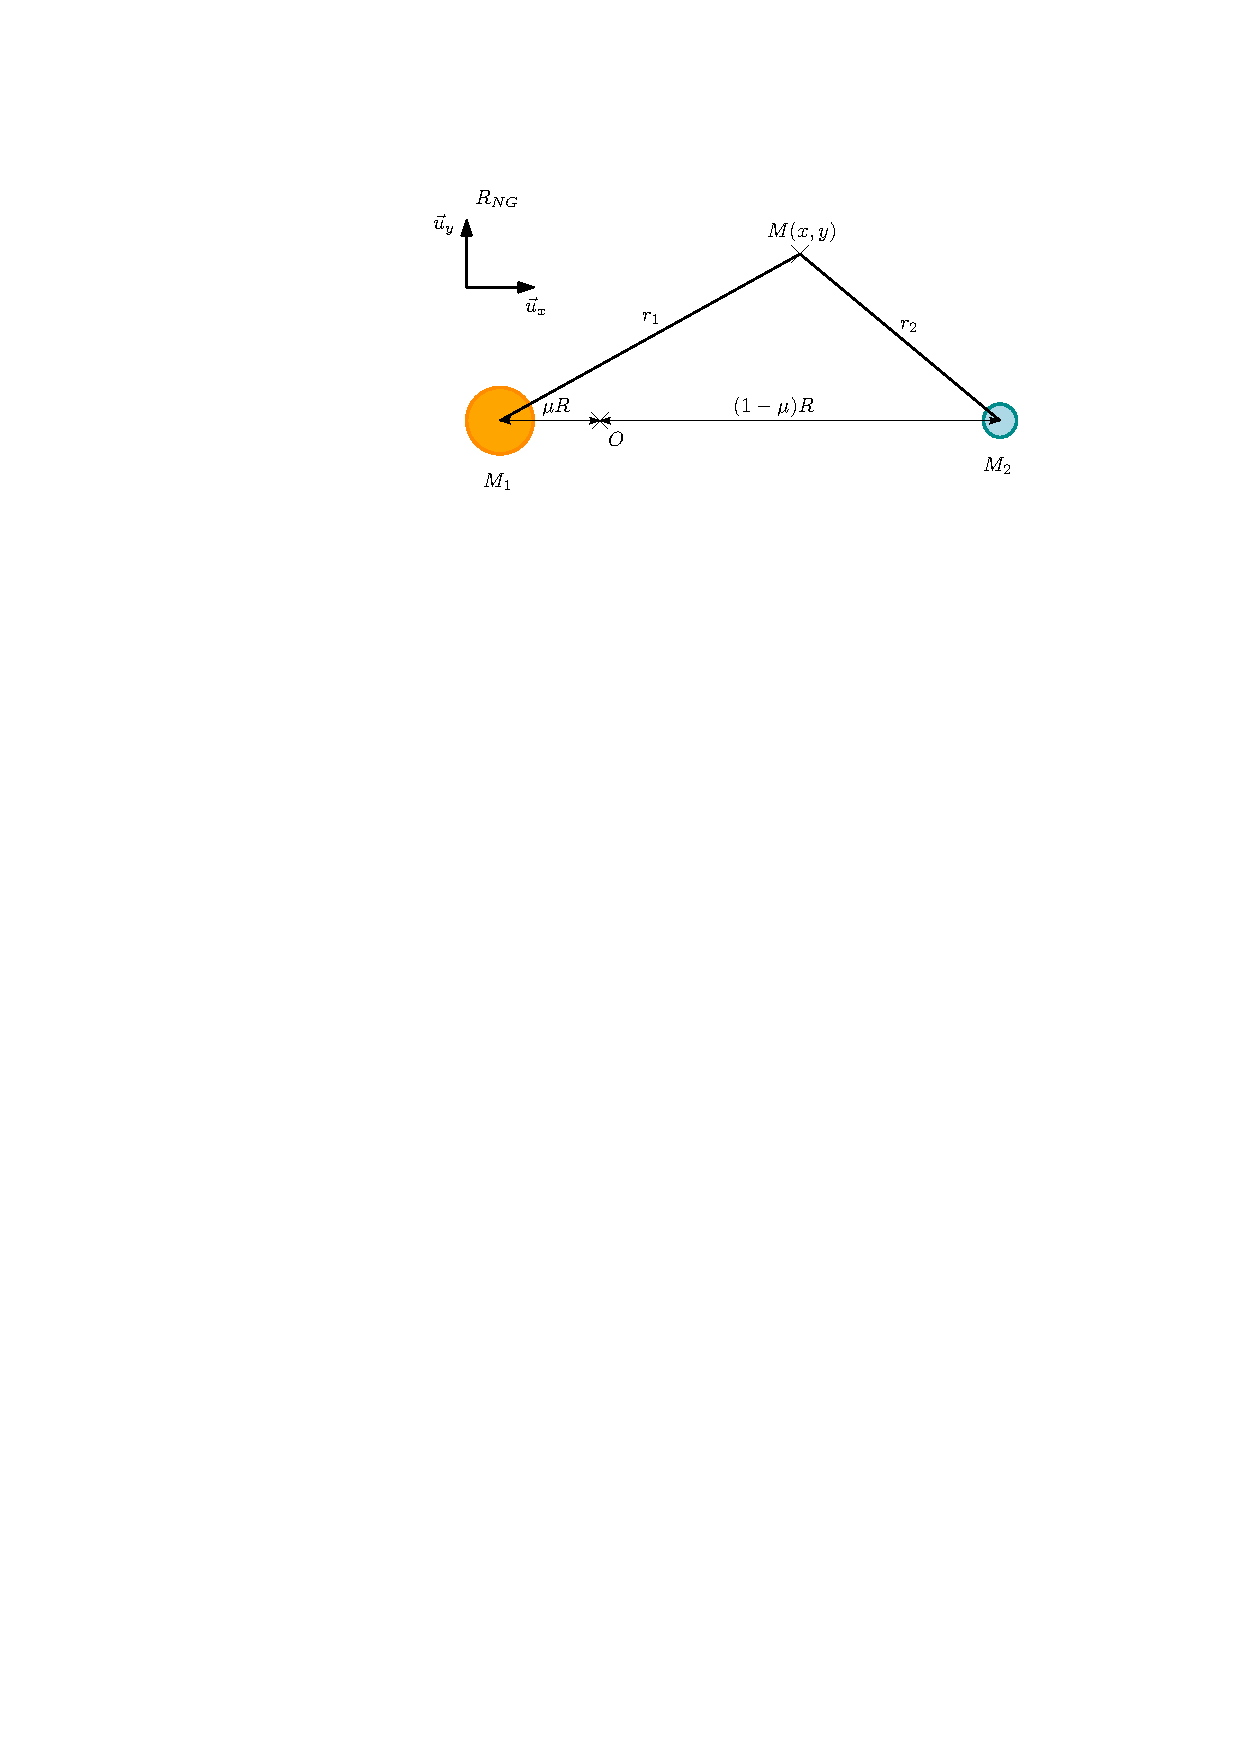
\includegraphics[width=0.75\linewidth]{ref_rng_diag.pdf}
				\caption{Schéma du référentiel $R_{NG}$.}
				\label{diagram rng}
		\end{figure}
	\end{frame}
	
	\begin{frame}
		Equations du mouvement dans $R_{NG}$ :
		\begin{equation*}
			\label{eq du mvt}
			\begin{cases}
				\ddot{x} - 2\omega\dot{y} = - \frac{1}{m}\bar{\mathcal{U}}_x \\
				\ddot{y} + 2\omega\dot{x} = - \frac{1}{m}\bar{\mathcal{U}}_y
			\end{cases}
		\end{equation*}
		
		et on en déduit le potentiel effectif dans $R_{NG}$ :
		\begin{tcolorbox}[colframe=black,boxrule=0.8pt,colback=white]
			\begin{equation}
				\bar{U} = U(x,y) - \frac{1}{2}m\omega^2(x^2+y^2)
			\end{equation}
		\end{tcolorbox}
	\end{frame}
	
	\begin{frame}
		\begin{figure}
			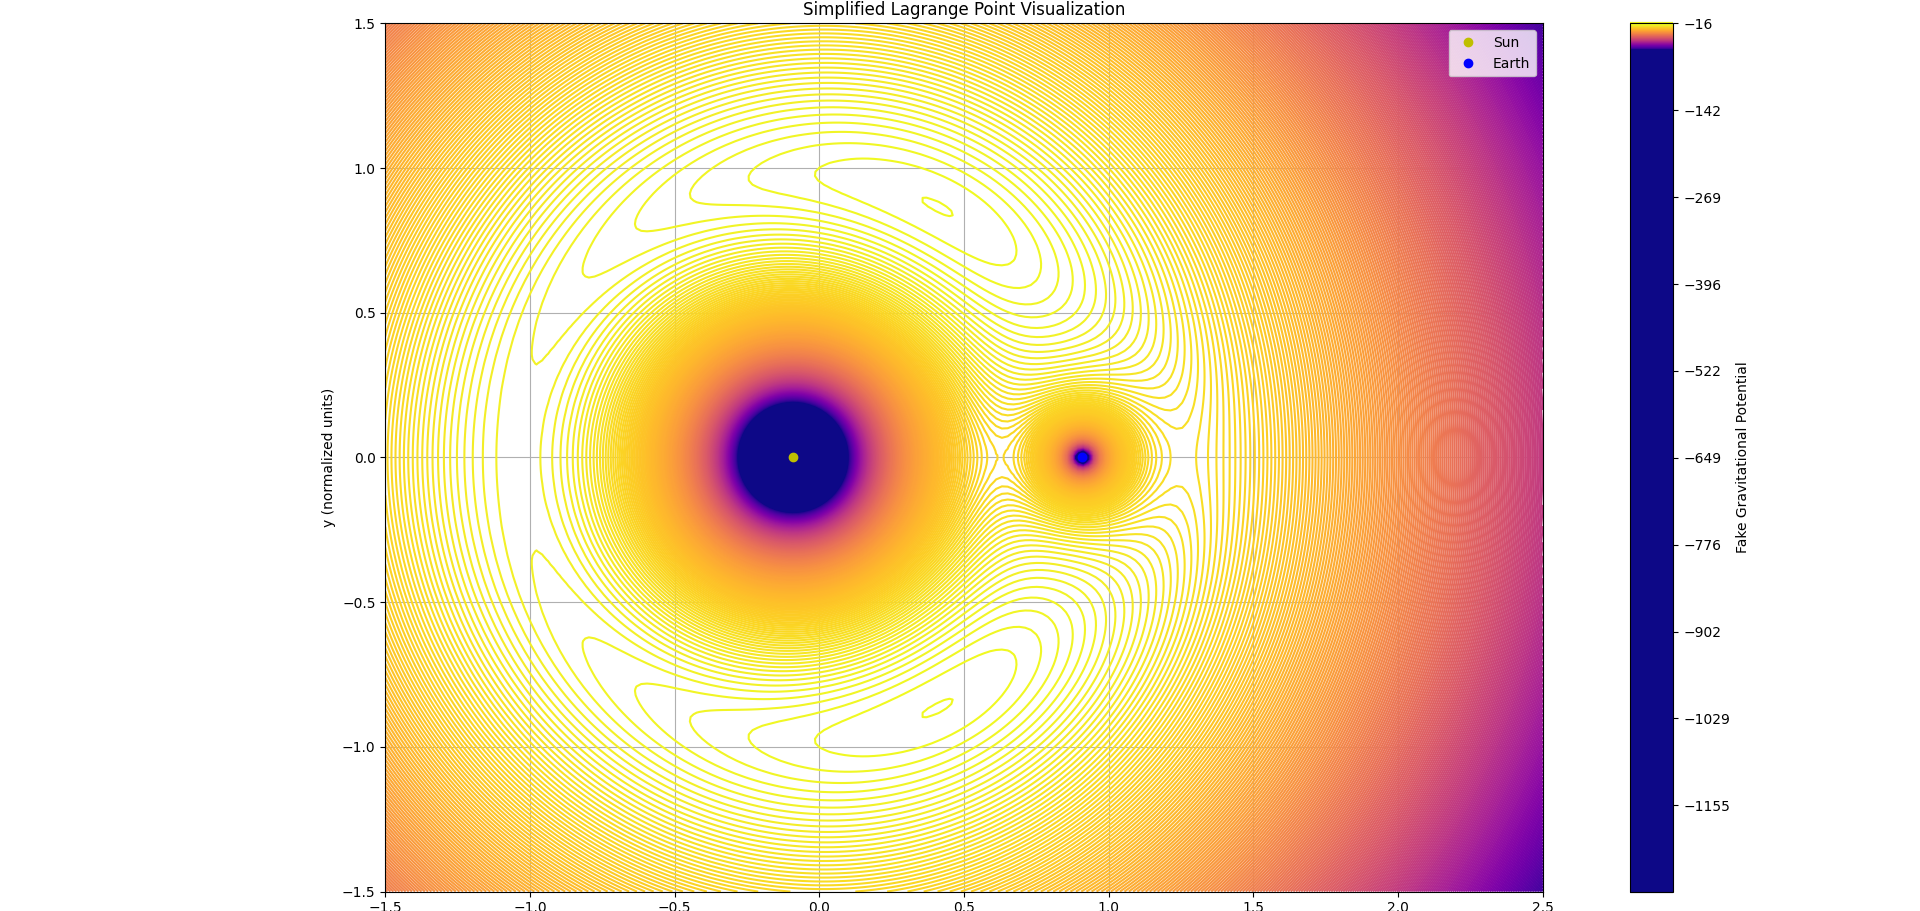
\includegraphics[width=1\linewidth]{potential_clear.png}
			\caption{Tracé du potentiel effectif $\bar{U}$ en Python (cf. Annexe \ref{python tracé potentiel}).}
			\label{tracé du potentiel 3D python}
		\end{figure}
	\end{frame}
	
	
	
	\subsection{Coordonnées des points colinéaires}
	\begin{frame}
		On cherche des solutions en $y=0$. Le potentiel devient
		\begin{equation*}
			\label{potential_in_y=0}
			\bar{U}(x,0)=-\frac{1}{2}m\omega^2x^2-\frac{GmM_1}{|x+\mu R|}-\frac{GmM_2}{|x-(1-\mu)R|}
		\end{equation*}
		avec $\mu := \frac{M_2}{M_1+M_2}$.
		\begin{figure}
			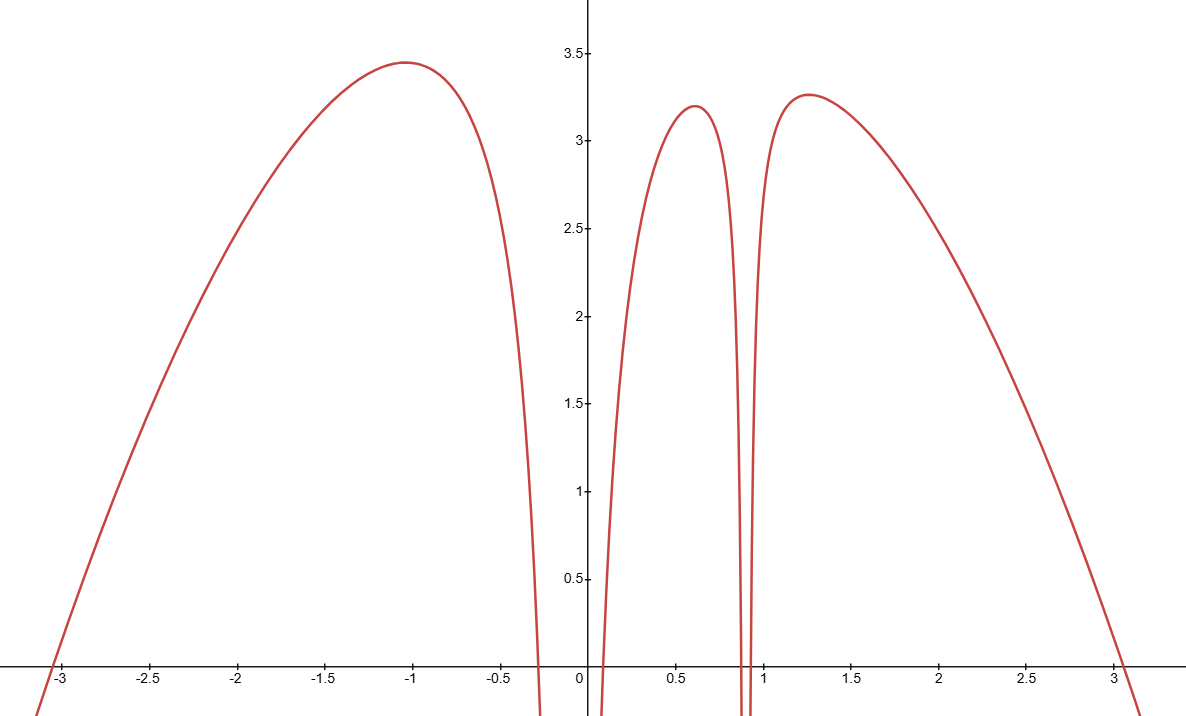
\includegraphics[width=0.4\linewidth]{graphe_potentiel_en_x}
			\caption{Tracé du potentiel effectif $x \mapsto \bar{U}(x,0)$ avec Desmos.}
			\label{tracé du potentiel 3D python}
		\end{figure}
	\end{frame}
	
	\begin{frame}
		\begin{equation*}
			(E) \ \ \frac{\partial \bar{U}}{\partial x}(x,0) = 0, \text{ d'inconnue } x \in \mathbb{R}
		\end{equation*}
		En supposant $\mu \to 0$, on obtient
			
		\begin{table}[H]
			\centering
			\label{tab:points_colinéaires_coord}
			\renewcommand{\arraystretch}{1.6}
			\begin{tabular}{|c|c|c|}
				\hline
				Point & Coordonnée en $x$ & Coordonnée en $y$
				\\ \hline
				L1 & $((1-\mu) - (\frac{\mu}{3})^{\frac{1}{3}})R$ & 0
				\\ \hline
				L2 & $((1-\mu) + (\frac{\mu}{3})^{\frac{1}{3}})R$ & 0
				\\ \hline
				L3 & $(-1-\frac{5\mu}{12})R$ & 0
				\\ \hline
			\end{tabular}
			\caption{Coordonnées des points colinéaires.}
		\end{table}		
	\end{frame}
	
	
	\subsection{Coordonnées des points équilatéraux}
	\begin{frame}
		On cherche des points d'équilibre pour $y \neq 0$. On a dans ce cas
		\begin{equation*}
			\label{equi_underived_eq}
			\begin{cases}
				r_1=\sqrt{(x+\mu R)^2+y^2}
				\\ r_2 = \sqrt{(x-(1-\mu)R)^2+y^2}
				\\ \bar{U}(x,y)=-\frac{1}{2}m\omega^2(x^2+y^2)-\frac{GmM_1}{r_1}-\frac{GmM_2}{r_2}
			\end{cases}
		\end{equation*}
		et on veut les points où les deux dérivées suivantes s'annulent :
		\begin{equation*}
			\label{equi_derived_eq}
			\begin{cases}
				\frac{\partial \bar{U}}{\partial x} = -m\omega^2x+\frac{GmM_1(x+\mu R)}{r_1^3}+\frac{GmM_2(x-(1-\mu)R)}{r_2^3}
				\\
				\frac{\partial \bar{U}}{\partial y} = -m\omega^2y+\frac{GmM_1y}{r_1^3}+\frac{GmM_2y}{r_2^3}
			\end{cases}
		\end{equation*}
		
		Cela impose $r_1 = r_2 = R$.
	\end{frame}
	
	\begin{frame}
		\begin{table}[H]
			\centering
			\label{tab:toutes_les_coord}
			\renewcommand{\arraystretch}{1.6}
			\begin{tabular}{|c|c|c|}
				\hline
				Point & Coordonnée en $x$ & Coordonnée en $y$
				\\ \hline
				L1 & $((1-\mu) - (\frac{\mu}{3})^{\frac{1}{3}})R$ & 0
				\\ \hline
				L2 & $((1-\mu) + (\frac{\mu}{3})^{\frac{1}{3}})R$ & 0
				\\ \hline
				L3 & $(-1-\frac{5\mu}{12})R$ & 0
				\\ \hline
				L4 & ($(\frac{1}{2}-\mu)R$) & $\frac{\sqrt{3}}{2}R$
				\\ \hline
				L5 & ($(\frac{1}{2}-\mu)R$) & $-\frac{\sqrt{3}}{2}R$
				\\ \hline
			\end{tabular}
			\caption{Coordonnées des points de Lagrange.}
		\end{table}	
	\end{frame}
	
	
	\begin{frame}
		\begin{figure}
			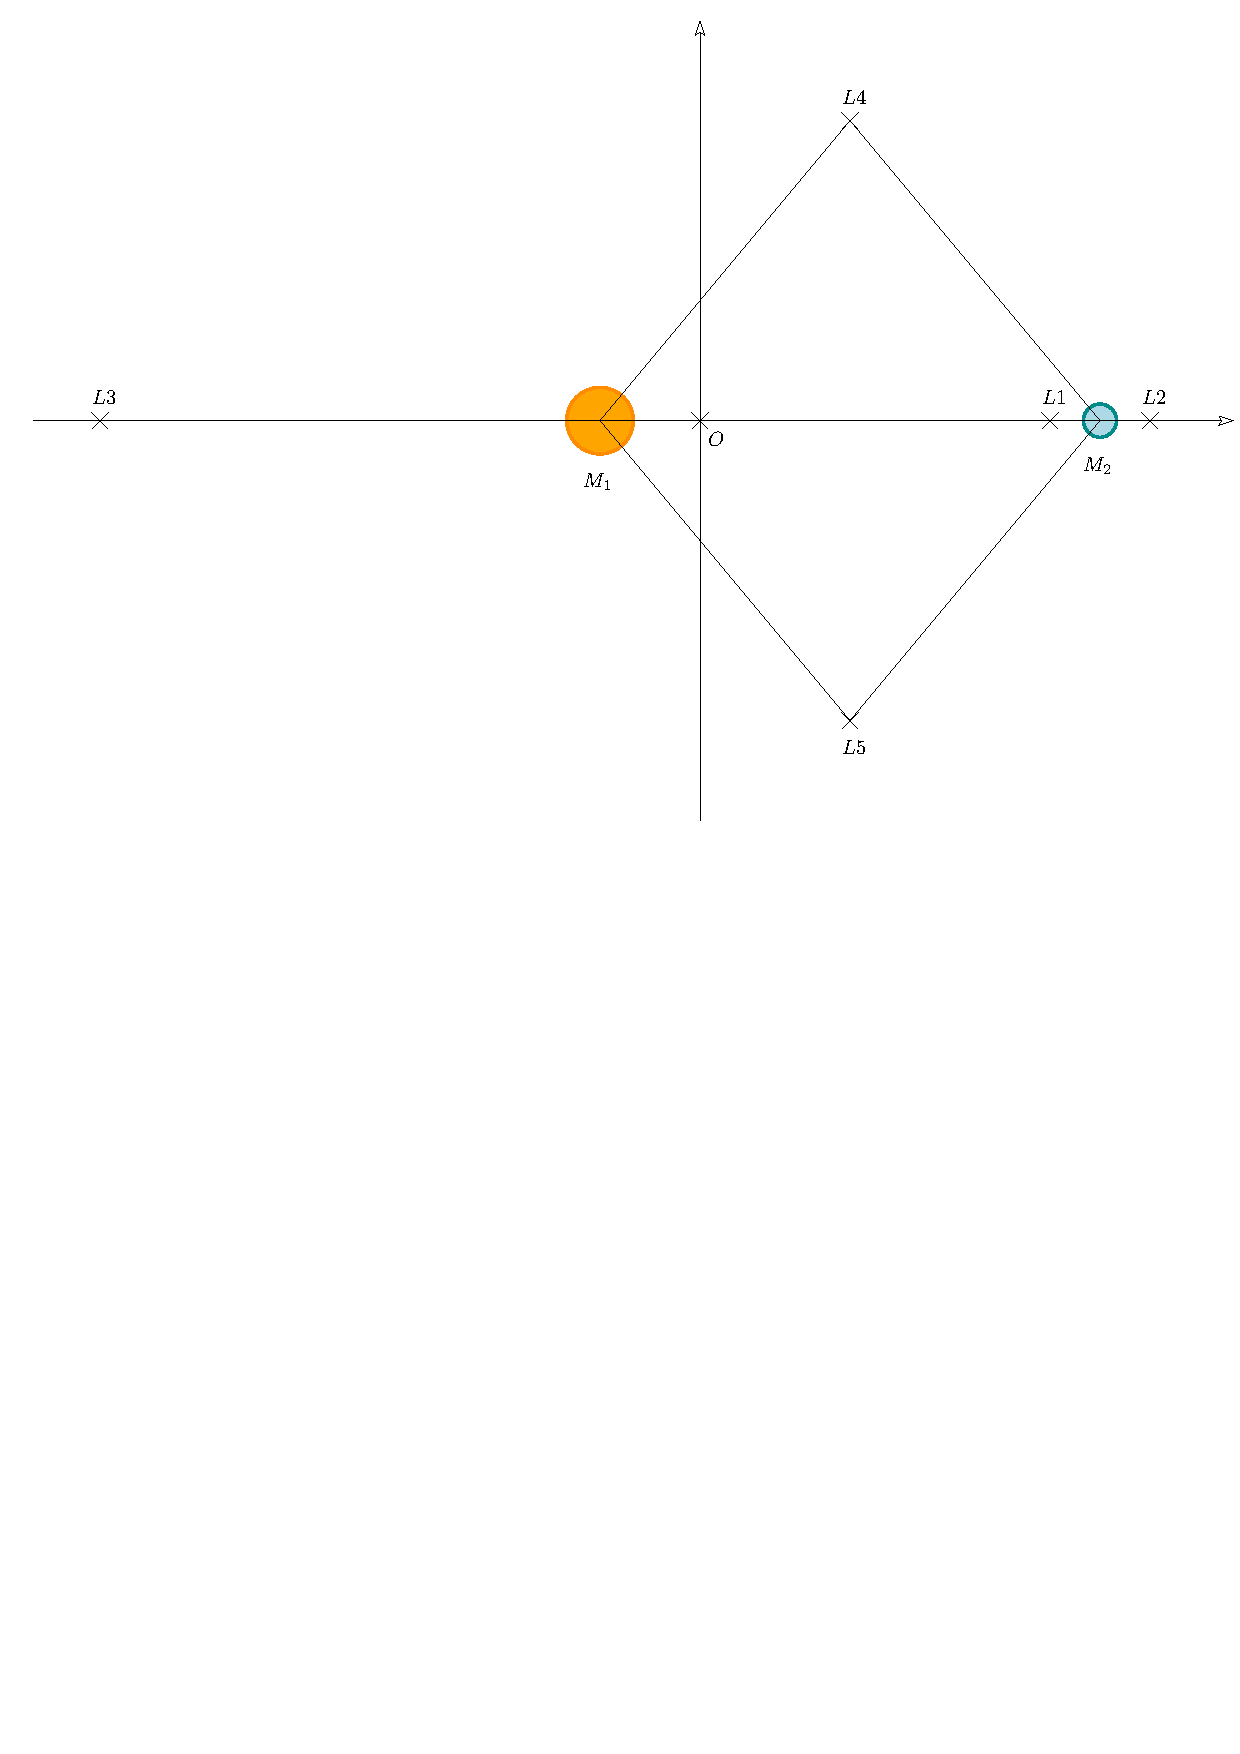
\includegraphics[width=0.8\linewidth]{ref_rng_avec_points_deq.pdf}
			\caption{Schéma de $R_{NG}$ avec les points de Lagrange.}
			\label{ref rng avec les points d'équilibre}
		\end{figure}
	\end{frame}
	
	
	
	
	
	\section{Stabilité des points de Lagrange}
	\subsection{Linéarisation des équations du mouvement}
	\begin{frame}
		Les équations du mouvements sont
		\begin{equation*}
			\label{équations du mouvement}
			\begin{cases}
				\dot{x} = v_x
				\\
				\dot{y} = v_y
				\\
				\dot{v_x} = \ddot{x} = 2\omega\dot{y} - \frac{1}{m}\bar{\mathcal{U}}_x
				\\
				\dot{v_y} = \ddot{y} = - 2\omega\dot{x} - \frac{1}{m}\bar{\mathcal{U}}_y
			\end{cases}
		\end{equation*}
		ce qui se linéarise en
		\begin{equation*}
			\begin{bmatrix}
				0 & 0 & 1 & 0 \\
				0 & 0 & 0 & 1 \\
				-\frac{1}{m}\bar{\mathcal{U}}_{xx}^i & -\frac{1}{m}\bar{\mathcal{U}}_{xy}^i
				& 0 & 2\omega \\
				-\frac{1}{m}\bar{\mathcal{U}}_{yx}^i & -\frac{1}{m}\bar{\mathcal{U}}_{yy}^i
				& -2\omega & 0
			\end{bmatrix}
			=: A
		\end{equation*}
		où $\mathcal{\bar{U}}_{wz}^i = \frac{\partial ^2\bar{U}}{\partial w \partial z}(x_{L_i}, y_{L_i})$
	\end{frame}
	
	
	
	
	
	
	
	
	
	
	
	
\end{document}